\documentclass[12pt, letterpaper, twoside]{article}
\usepackage{nopageno,epsfig, amsmath, amssymb}
\usepackage{physics}
\usepackage{mathtools}
\usepackage{hyperref}
\usepackage{xcolor}
\usepackage{array}
\hypersetup{
    colorlinks,
    linkcolor={blue},
    citecolor={blue},
    urlcolor={blue}
}
\usepackage{empheq}
\usepackage{wrapfig}

\usepackage[letterpaper,
            margin=0.8in]{geometry}

\newcommand{\psetnum}{6}
\newcommand{\class}{ASTR 541 - Interstellar Medium}

\newcommand{\tomtitle}{
    \noindent {\LARGE \fontfamily{cmr}\selectfont \textbf{\class}} \hfill \\[1\baselineskip]
    \noindent {\large \fontfamily{cmr}\selectfont Problem Set \psetnum \hfill \textsc{Tom Wagg}}\\[0.5\baselineskip]
    {\fontfamily{cmr}\selectfont \textit{\today}}\\[2\baselineskip]
}

\title{\class : Week \psetnum}
\author{\textbf{Tom Wagg}}

\newcommand{\question}[1]{{\noindent \it #1}}
\newcommand{\answer}[1]{
    \par\noindent\rule{\textwidth}{0.4pt}#1\vspace{0.5cm}
}
\newcommand{\todo}[1]{{\color{red}\begin{center}TODO: #1\end{center}}}

% custom function for adding units
\makeatletter
\newcommand{\unit}[1]{%
    \,\mathrm{#1}\checknextarg}
\newcommand{\checknextarg}{\@ifnextchar\bgroup{\gobblenextarg}{}}
\newcommand{\gobblenextarg}[1]{\,\mathrm{#1}\@ifnextchar\bgroup{\gobblenextarg}{}}
\makeatother

\newcommand{\avg}[1]{\left\langle #1 \right\rangle}
\newcommand{\angstrom}{\mbox{\normalfont\AA}}
\allowdisplaybreaks

\newcolumntype{C}{>{$}c<{$}}

\begin{document}

\tomtitle{}

\noindent For reference, if you'd ever like to see the code that I've used to get my answers to these, \href{https://github.com/TomWagg/uw-grad-classes/tree/main/541_ism}{here's a link to my GitHub repo}! (\#astropy.units for life)\\


\question{\textbf{1. Spectroscopy}}
\answer{
    I'm going to summarise my results in a single table to make it a bit easier to parse.
    \begin{center}
        \boxed{
        \begin{tabular}{l|c|c|c|c|c|c}
            Galaxy & Redshift & SII Ratio & O3HB & N2 & O3N2 & Oxygen Abundance \\
            \hline
            J0929+4644\_172\_157 & 0.017 & 1.27 & 5.45 & 0.05 & 2.06 & 8.17 \\
            J0943+0531\_106\_34 & 0.228 & 1.30 & 0.43 & 0.55 & -0.11 & 8.77
        \end{tabular}}
    \end{center}
    \textbf{Density regimes:} Both of these galaxies are in a low density regime since the SII ratios are both close to 1.44 (which we calculated in the last homework).\\

    \noindent \textbf{Spectrum Noise:} The second galaxy is noisier because it is at a higher redshift and therefore all fluxes are lower.\\

    \noindent \textbf{Galaxy Masses:} The second galaxy has a higher oxygen abundance. Therefore I think this means that \textbf{the second galaxy must be more massive}. The reason for this is that massive stars enrich the gas and increase the oxygen abundance. So a higher stellar mass would result in a larger oxygen abundance.
}

\question{\textbf{2. HII Heating and Cooling Balance}}

\question{2a. Heating}
\answer{
    The main source of heating is the photoionisation. The energy of the photons is transferred into ionising the hydrogen and the leftover kinetic energy that the electrons gains leads to heating of the gas. The heating rate due to this can be written as follows
    \begin{equation}
        \boxed{\Gamma_{\rm ion, H} = \underbrace{\vphantom{\frac{3}{2} k_B T_{\rm init}} n_e n_p}_{(1)} \underbrace{\vphantom{\frac{3}{2} k_B T_{\rm init}} \alpha_B(T)}_{(2)} \underbrace{\frac{3}{2} k_B T_{\rm init}}_{(3)}}
    \end{equation}
    Where (1) shows the density of ``things that could be ionised'', i.e. the hydrogen, and the density of electrons. (2) is the total recombination coefficient which has the temperature dependence and indicate the rate at which recombination occurs. (3) is the average initial kinetic energy.
}

\clearpage

\question{2b. Cooling}
\answer{
    A large source of cooling is recombination, this cooling rate can be written as follows. We can also convert $\beta_H(T)$ to $\alpha_B(T)$ using the expression given in the question.
    \begin{align}
        \Lambda_{\rm recomb, H} &= n_e n_p k_B T \beta_H(T)\\
        \Aboxed{ \Lambda_{\rm recomb, H} &= 0.86 n_e n_p k_B T \alpha_B(T) }
    \end{align}
    $\beta_H(T)$ is the likelihood that an electron will be reabsorbed per energy (and includes the maxwellian distribution), $k_B T$ gives the energy based on the temperature and the densities indicate how often we find electrons to be reabsorbed and protons with which to recombine.
}

\question{2c. Balance}
\answer{
    Now we can equate the heating rate from part (a) and the cooling rate from part b (plus the free-free emission) and reduce the equation.
    \begin{align}
        n_e n_p \alpha_B(T) \cdot \frac{3}{2} k_B T_{\rm init} &= 0.86 n_e n_p k_B T \alpha_B(T) + 0.54 n_e n_p \alpha_B(T) \qty(\frac{T}{10^4 \unit{K}})^{0.37} k_B T \\
        \alpha_B(T) \cdot \frac{3}{2} T_{\rm init} &= 0.86 T \alpha_B(T) + 0.54 \alpha_B(T) \qty(\frac{T}{10^4 \unit{K}})^{0.37} T \\
        \Aboxed{\frac{3}{2} T_{\rm init} &= T \qty[0.86  + 0.54 \qty(\frac{T}{10^4 \unit{K}})^{0.37}]}
    \end{align}
}

\question{2d. Solve it!}
\answer{
    Using \href{https://docs.scipy.org/doc/scipy/reference/generated/scipy.optimize.fsolve.html}{\texttt{scipy.optimize.fsolve}}, I found that the equilibrium temperature is
    \begin{equation}
        \boxed{ T = 28918 \unit{K} }
    \end{equation}
}

\question{2e. Metal Lines}
\answer{
    Metal line transitions would lead to addition cooling and produce an extra term for the cooling side of the balance equation. Each potential metal transition allows a different photon energy to absorbed and then re-emit. Many of the forbidden line transitions can then produce photons that escape easily and lead to cooling.

    This will additionally work differently in different density regimes. At low density there is a stronger ($n^2$) dependence on number density, but at higher density this weakens to a linear scaling with $n$.
}

\clearpage

\question{Bonus round - OII cooling}
\answer{
    Congratulations - by making it this far through the problem set you've unlocked a secret bonus round! Let's investigate how the cooling from a particular OII transition could change things in a cloud with a nonzero metallicity.

    \noindent Imagine that we have an HII region with solar abundance of oxygen (but somehow no other metals) and let's just focus on a particular transition that Jess indicated would be important. Additionally, let's just operate in the low density regime (which is maybe reasonable at this temperature? Either way I'm doing it to help the algebra :p).\\

    \noindent Okay now let's rebalance our heating and cooling with an additional term for the low-density metal line cooling from OII.
    \begin{equation}
        \frac{3}{2} T_{\rm init} = T \qty[0.86 + 0.54 \qty(\frac{T}{10^4 \unit{K}})^{0.37}] + \underbrace{f_{O/H} \gamma_{lu}(T) \frac{h \nu_{ul}}{k_B \alpha_B(T)}}_{\text{this is the new bit}}
    \end{equation}
    Nice! Now we need to define all of these delightfully delectable terms. $f_{O/H}$ is the relative number density of oxygen to hydrogen in the Sun, looking this up online\footnote{\url{http://hyperphysics.phy-astr.gsu.edu/hbase/Tables/suncomp.html}} I found that
    \begin{equation}
        f_{O/H} = 0.043 / 91.2 = 4.7 \times 10^{-4}
    \end{equation}
    It would now be useful to consider which transition we are focussing on (it's about to be relevant), so we can use my final project to work out the spectroscopic terms of OII and plot up its energy level diagram (with some transitions grabbed from Draine):
    \begin{center}
        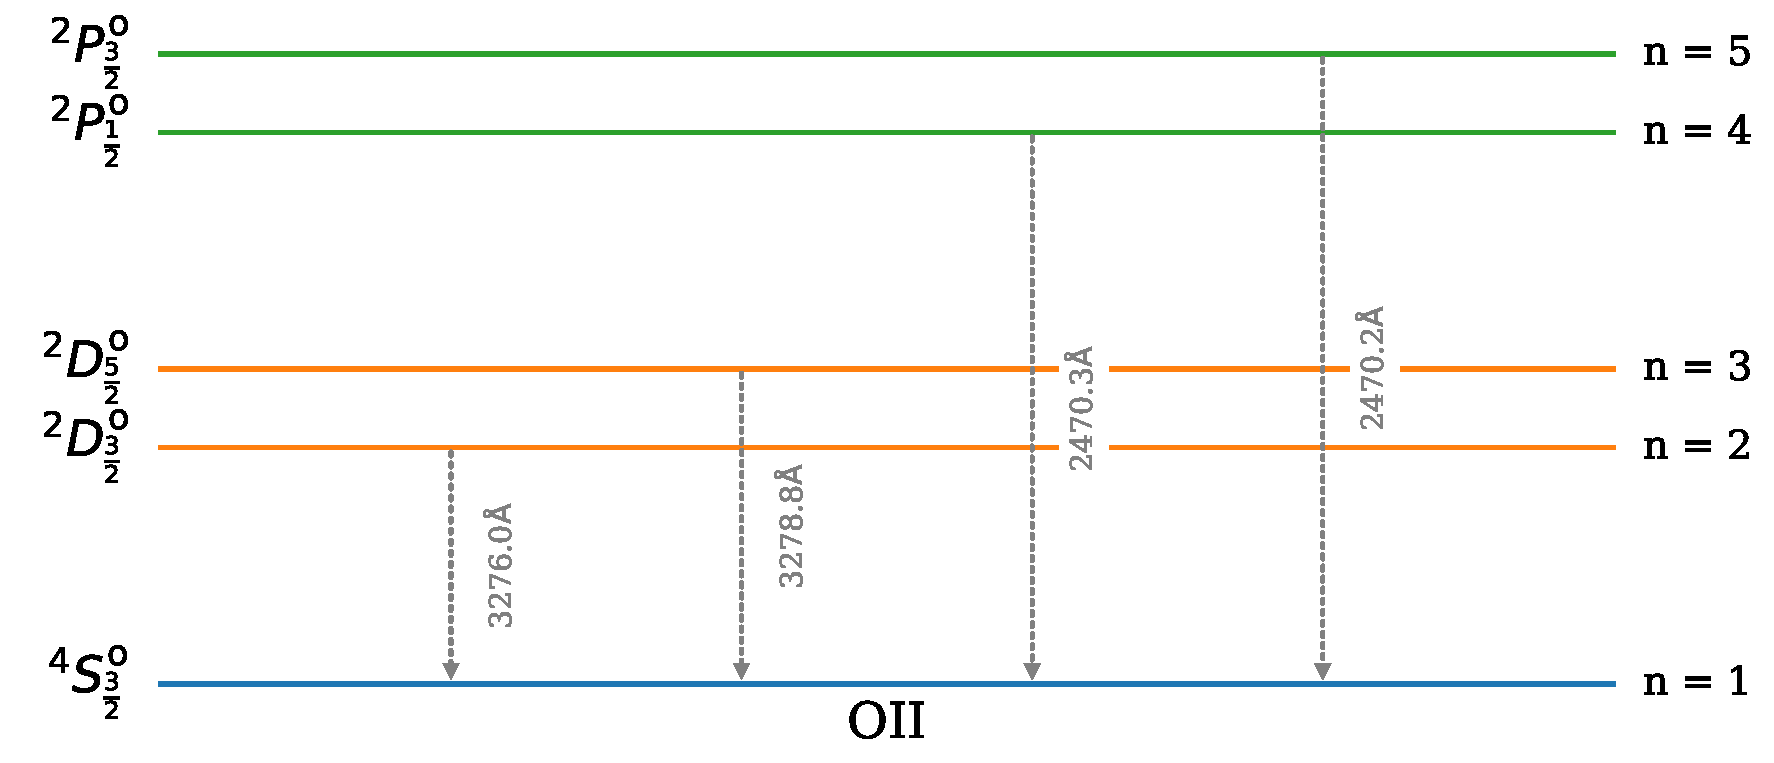
\includegraphics[width=0.8\textwidth]{OII_levels.pdf}
    \end{center}
    We're going to focus on the second transition shown here with a wavelength of $\lambda = 3278.8 \unit{\AA}$. Draine gives (in Table F.4) that, for this transition,
    \begin{equation}
        \Omega_{ul} = 0.803 T_4^{0.023 - 0.008 \ln T_4},
    \end{equation}
    where $T_4 = T / 10^4 \unit{K}$. In lecture 5 (towards the end) we related $\Omega_{ul}$ to $\gamma_{ul}$ as
    \begin{equation}
        \gamma_{ul} = \frac{\Omega_{ul}}{g_u} \frac{h^2}{(2 \pi m_e)^{3/2} (k_B T)^{1/2}}
    \end{equation}
    And in this case $g_u = 2 (5/2) + 1 = 6$. Okay hang in there, just two more terms (and they're easier!). Given the transition wavelength, we immediately have the energy:
    \begin{equation}
        h \nu_{ul} = \frac{h c}{\lambda_{ul}} = 3.33 \unit{eV}
    \end{equation}
    And we are given an expression for $\alpha_B(T)$ in the question
    \begin{equation}
        \alpha_B(T) = 4 \times 10^{-13} \unit{cm^3}{s^{-1}} T_4^{-0.73}
    \end{equation}
    And that's everything we need! We can summarise at the new cooling rate from OII
    \begin{align}
        \Lambda_{\rm OII} &= 4.7 \times 10^{-4} \qty(0.803 T_4^{0.023 - 0.008 \ln T_4}) \frac{1}{6} \frac{h^2}{(2 \pi m_e)^{3/2} (k_B T)^{1/2}} \frac{h c}{\lambda k_B} \cdot 2.5 \times 10^{12} \unit{cm^{-3}}{s} T_4^{0.73} \\
        \Lambda_{\rm OII} &= \qty[1.57 \times 10^{8} \frac{h^3 c}{\lambda (2 \pi m_e)^{3/2} k_B^{3/2}}\cdot \unit{cm^{-3}}{s}] \cdot T_4^{0.753 - 0.008 \ln T_4} T^{-1/2}
    \end{align}\\

    \noindent Now it \emph{should} be as easy as plugging this into the same Python function as before...but sadly \textbf{there seems to be a mistake somewhere} because it crashes. When we were doing this at the end of class, we just added units to the $\Omega_{ul}$ terms which I don't think is valid given the conversion that I found in the lecture notes. This allowed us to find a temperature of a couple thousand Kelvin.

    In reality, if I plug in this expression, the cooling seems to be so large that there is no positive temperature solution. I'd be very intrigued to hear what I did wrong here!
}

\end{document}

 